\documentclass{article}
\usepackage{amsmath,amssymb}
\usepackage{algorithm,algorithmic}
\usepackage{graphicx}
\usepackage{listings}
\usepackage{color}
\usepackage[margin=1in]{geometry}
\usepackage[colorlinks]{hyperref}
%\usepackage{fullpage}

\definecolor{dkgreen}{rgb}{0,0.6,0}
\definecolor{gray}{rgb}{0.5,0.5,0.5}
\definecolor{mauve}{rgb}{0.58,0,0.82}

\lstset{frame=tb,
  language=Java,
  aboveskip=3mm,
  belowskip=3mm,
  showstringspaces=false,
  columns=flexible,
  basicstyle={\small\ttfamily},
  numbers=none,
  numberstyle=\tiny\color{gray},
  keywordstyle=\color{blue},
  commentstyle=\color{dkgreen},
  stringstyle=\color{mauve},
  breaklines=true,
  breakatwhitespace=true
  tabsize=0
}
\begin{document}


\title{\textbf{CS3410: Software Engineering Lab}\\ \textbf{LR(1) parser for JavaCC}}
\author{
	Srinivasan R CS11B059 \\
	Aravind S CS11B033\\
    Akshayaram S CS11B057 \\
    Ramnandan SK CS11B061 \\
    Adit Krishnan CS11B063
}

\maketitle
\section{Introduction}
In this project, we built a LR(1) parser generator for JavaCC. Currently, JavaCC generates LL(k) parser. The main drawback with LL(k) grammars is that it cannot parse left recursive grammars. Though, there are algorithms to convert left recursive grammars to non-left recursive case, they lead to an explosion in the number of productions and hence such algorithms are inefficient. On the other hand, LR(1) parsers can parse all LL(k) grammars and left recursive grammars with minimal space and time overhead. 

\section{Cohesion and Coupling}
The parser code for the JavaCC parser was located in the src/org/javacc/parser/. Though we had to make changes to one file and add two files to the folder, we had to comprehensively study all the 66 files present in the parser folder in order to fully understand the data abstraction and the control flow that was happening. As and when we went through the code, we made the following observations regarding the cohesion and coupling between modules.

\subsection*{Cohesion Analysis}
The functions within a module exhibited fairly high cohesion like functional or sequential cohesion. As far as we observed, we didn't find any instance of logical or coincidental cohesion in a function which are undesirable.

Even in the functions that we added to the src/org/javacc/parser/ParseEngine.java we ensured that they had functional or sequential cohesion. There were cases where we had to give different outputs depending on whether the token was a non-terminal or a terminal (eg. computeGoTo(), buildClosure()). But this would have lead to logical cohesion within the function. In order to avoid this we split the function and wrote separate functions for computeGoToRegEx() and computeGoToNonTerminal() which individually exhibit functional cohesion. 

\subsection*{Coupling Analysis}
In the parser folder, JavaCCGlobals.java contains global data structures which can be accessed by the rest of the parser module. Basically, it contains the list of constants, terminals which were observed during the lexical analysis. Hence, JavaCCGlobals.java has common coupling with other modules like ParseEngine.java and ParseGen.java. 

We were careful in not introducing any instance of common coupling between the modules where we made changes. All the data structures we used were local to a particular class and is not accessible else where. Hence, we introduced loose coupling within the modules where we made changes (At worst, we introduced stamp coupling within the modules where we made changes)   

To conclude, though parser files exhibit high levels of cohesion at a functional level, there are instances of common coupling which need to be avoided for better maintainability of the code.

\section{Class Hierarchies}
The main class hierarchies that were present in the parser file are shown below.
\begin{center}
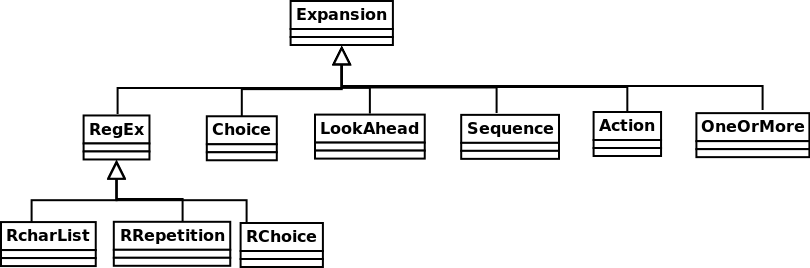
\includegraphics[scale=0.35]{Expansion.png}    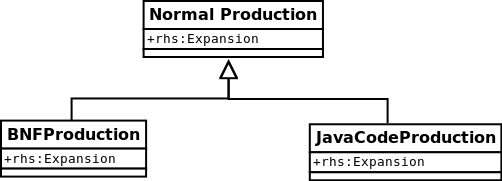
\includegraphics[scale=0.35]{NormalProduction.png} 
\end{center}

\begin{center}
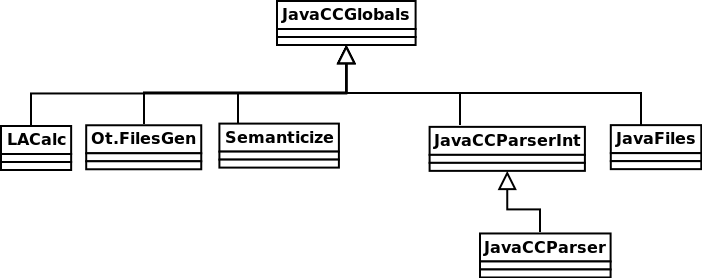
\includegraphics[scale=0.35]{javaCCGlobals.png}   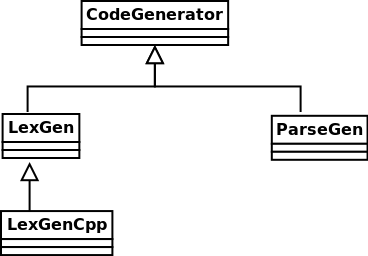
\includegraphics[scale=0.35]{CodeGenerator.png}
\end{center}

\section{Design Patterns}
There were not many design patterns that were present in the parser folder where we concentrated entirely. We could observe one instance of the builder  pattern and one instance of the factory method.
\begin{enumerate}
\item Builder Pattern :
The builder pattern we observed is shown below. 
\begin{center}
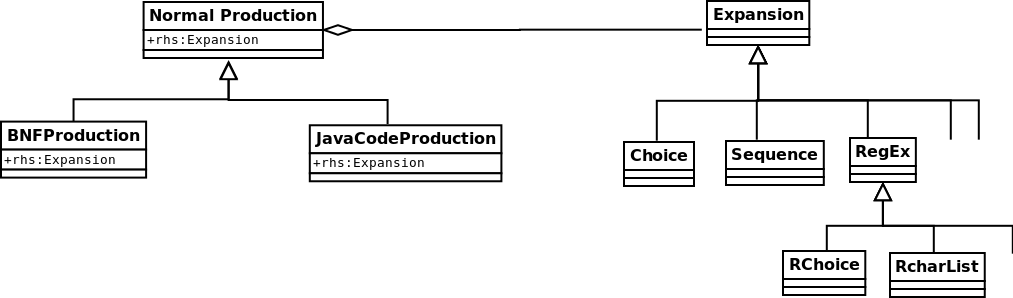
\includegraphics[scale=0.35]{builder1.png}
\end{center}
Based on the token that the Normal production gets from the lexical analyzer, there is a complex algorithm which decides which sub-class of the rhs expansion which must be instantiated. Hence, this is an instance of the builder pattern.
\item Factory Method :
The factory method we observed is shown below.
\begin{center}
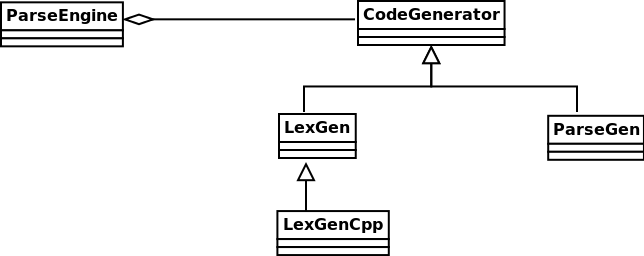
\includegraphics[scale=0.35]{FactoryMethod1.png}
\end{center}
Parse engine defines an interface for creating an object, but lets the subclasses of code generator to define which concrete class to instantiate at runtime depending on the context.
\end{enumerate}



\end{document}
